\subsection{Description of the objective}

The last step consists of modifying the client and the tracker in such a way that the client will not need a configuration file anymore. The client will instead try to discover the tracker by sending a broadcast message, and the tracker should respond to these discover requests.

\subsection{Proposed solution}

When launched, the tracker is listening to broadcast messages and to TCP requests in separated threads. This broadcast message is sent by the client when wanting to start a file download. The message is sent using UDP because this protocol does not require an established connection between the two agents.

\subsection{Sequence diagram}

The sequence diagram of the third step is shown in Figure \ref{fig:step3}.

The tracker now implements two threads, the first one listening to broadcast message and the second one handling TCP connection with the client as it did in step two.

\begin{figure}
	\centering
	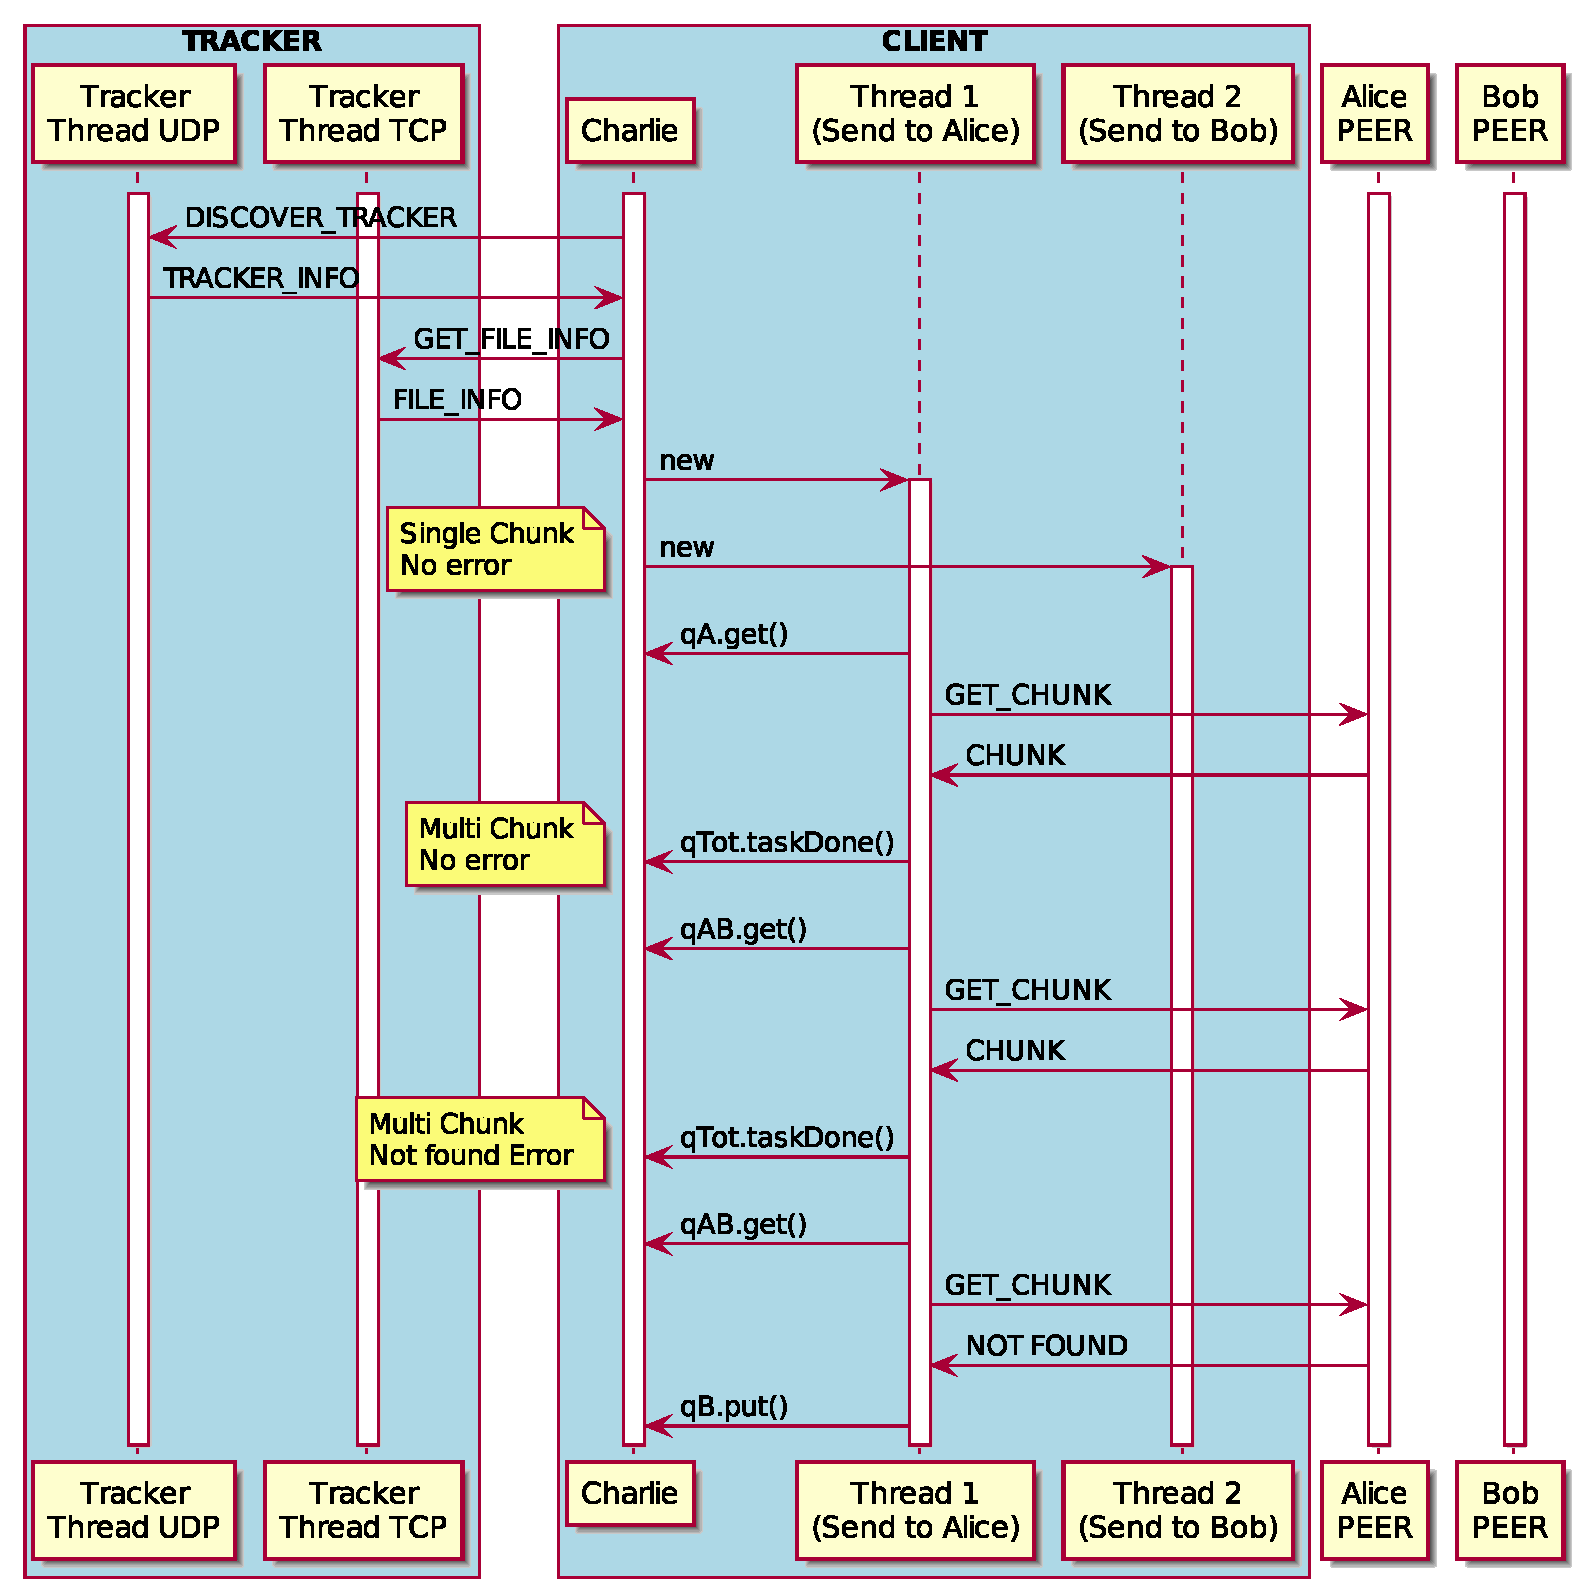
\includegraphics[width=\textwidth]{img/step3.eps}
	\caption{Sequence diagram of step 3}
	\label{fig:step3}
\end{figure}